\documentclass{article}
\usepackage[utf8]{inputenc}
\usepackage[T2A]{fontenc}
\usepackage[russian]{babel}
\usepackage{graphicx}
\usepackage{amsmath}
\usepackage{amssymb}
\usepackage{bm}
\usepackage[thinc]{esdiff}
\usepackage{mathtools}
\usepackage{breqn}
\usepackage{amsthm}
\usepackage{amsfonts}
\usepackage{bbm}

%Русская традиция
\renewcommand{\leq}{\leqslant}
\renewcommand{\geq}{\geqslant}
\renewcommand{\phi}{\varphi}
\DeclareMathOperator*{\argmax}{argmax}

\theoremstyle{definition}
\newtheorem{definition}{Определение}
\newtheorem*{definition*}{Определение}
\theoremstyle{theorem}
\newtheorem{theorem}{Теорема}
\theoremstyle{remark}
\newtheorem{remark}{Замечание}
\theoremstyle{theorem}
\newtheorem{corollary}{Следствие}
\theoremstyle{example}
\newtheorem{example}{Пример}
\theoremstyle{theorem}
\newtheorem{statement}{Утверждение}
\theoremstyle{theorem}
\newtheorem{alg}{Алгоритм}
\theoremstyle{theorem}
\newtheorem{sug}{Предположение}
\theoremstyle{theorem}
\newtheorem{lemma}{Лемма}

\begin{document}

\tableofcontents

\newpage

\section{ Компоненты свёрточной нейрнной сети}
	\begin{definition}
		Изображение~--- тензор $M\in\mathbb R^{m\times n\times d}$, $m$~--- ширина изображения, $n$~--- длина. Чаще всего $d=3$ (3 канала~--- Red, Green, Blue). 
	\end{definition}
	Учитывая, что обычно рассматривают трёхканальные или четырёхканальные изображения, можно под словом "тензор" понимать трёхмерный или четырёхмерный массив.
	
	Пусть $X \in\mathbb R^{m\times n\times d}$~--- случайная величина "изображение".
	
	Рассматриваются следующие задачи для изображений:
	\begin{itemize}
		\item Классификация $f:X\to\{1,\ldots,K\}$, $K$~--- число классов
		\item Сегментация (1 объект) $f:X\to Y$, $Y\in[0,1]^{m\times n}$, $Y_{ij}=\Prob(X_{ij}\in\text{segment})$, где $\text{segment}$~--- множество точек изображения (пикселей), принадлежащих объекту. Понятно, что можно обобщить на  сегментацию нескольких классов объектов.
	\end{itemize}
	\subsection{Свёртка}
		\begin{definition}
			Пусть $f,g:\mathbb R^n\to\mathbb R$, интегрируемые на $\mathbb R^n$. \textit{Свёрткой} будем называть функцию $f*g:\mathbb R^n\to\mathbb R$, равную $(f*g)(x)=\int\limits_{\mathbb R^n}f(y)g(x-y)dy$
		\end{definition}
		
		Далее под свёрткой будем понимать следующее определение.
		
		\begin{definition}
		Рассмотрим $M\in\mathbb{R}^{m\times n}$~--- изображение по одному из каналов, $K\in\mathbb R^{k\times l}$~--- ядро, \textit{свёрткой изображения относительно отображения $h:\mathbb{R}^{m\times n}\times\mathbb R^{k\times l}\to\mathbb R$ называется функция $*$}, рассмотрим, $(M*K)(i,j)=\sum\limits_{a=1}^k\sum\limits_{b=1}^l M_{i+a,j+b}K_{ab}$. $(M*K)\in\mathbb R^{(m-k+1)\times(n-l+1)}$
	\end{definition}
	
	Для того чтобы размер изображения после свёртки был равен исходному изображению можно как-нибудь заполнить края изображения (padding). Идея аналогична скользящему среднему с синхронизацией в центральной точке. 
	 В основном используются следующие способы padding:
	 \begin{itemize}
	 	\item zeros --- заполнение нулями.
	 	\item reflect --- "отражение", например, вектор $(1,2,3)$ при padding размера 2 отобразится в вектор $(3,2,1,2,3,2,1)$.
	 	\item replicate --- заполнение крайними значениями.
	 	\item circular --- круговое заполнение, вектор $(1,2,3)$ преобразуется в $(2,3,1,2,3,1,2)$.
	 \end{itemize}
	 \newpage
	 \begin{figure}[h!]
	 	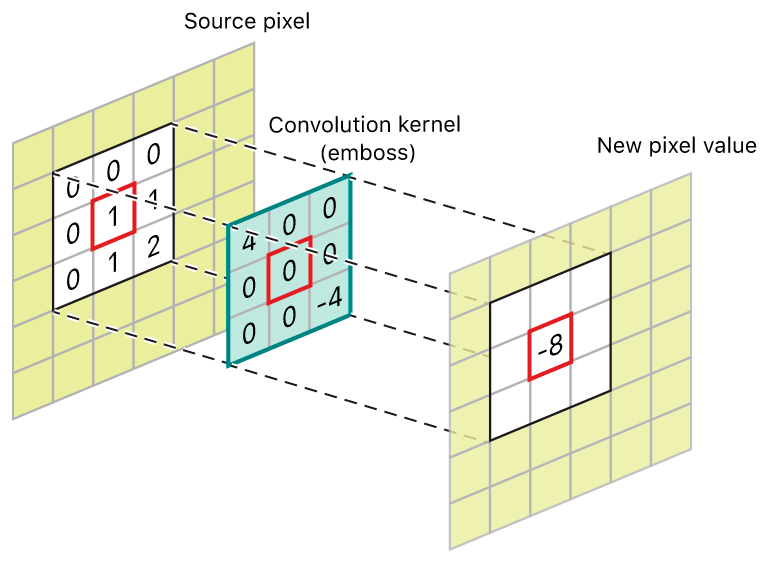
\includegraphics[width=\textwidth]{img/conv.png}\caption{Операция свёртки}
	 \end{figure}
	 \subsection{Свёрточный слой}
	 	Свёрточный слой задаётся следующими параметрами:
	 	\begin{itemize}
	 		\item Размер ядер $k\times l$ , $k\leq m$, $l\leq n$, $r\in\mathbb N$ число ядер
	 		\item Способ заполнения краёв (padding)
	 		\item Размер заполнения краёв $P\in \mathbb N_0$
	 		\item Величина сдвига ядра (stride) $S\in R^2$. Например, для $S=(1,1)$ получаем операцию, похожую на операцию вложения в 2D-SSA.
	 	\end{itemize}
	 \subsection{ Pooling слой}
	 	Свёрточная нейросеть помимо свёрточных слоёв состоит из pooling слоёв
	 	\begin{definition}
	 		Рассмотрим одноканальное изображение (матрицу)  $M$ размера $m\times n$. Выберем $p$ и $q$, кратные $m$ и $n$ соответственно. Разобьём матрицу на дизъюнктные подматрицы размера $k\times l$ $P_{ij}=\{M_{(i-1)p+k,(j-1)q+l}\}_{k=1,l=1}^{p,q}$, $i\in1:\frac mp$, $j\in1:\frac nq$. \textit{Операция pooling} применяет к каждой матрице $P_{ij}$ некоторую функцию $f$, в результате получается матрица $F$, состоящая из элементов $F(i,j)=f(P_{ij})$.
	 	\end{definition}
	 	
	 	Чаще всего используют max pooling, average pooling и sum pooling.
	 		Pooling слой применяется для уменьшения размерности изображения.
	 	\begin{figure}[ht!]\label{pool}
	 		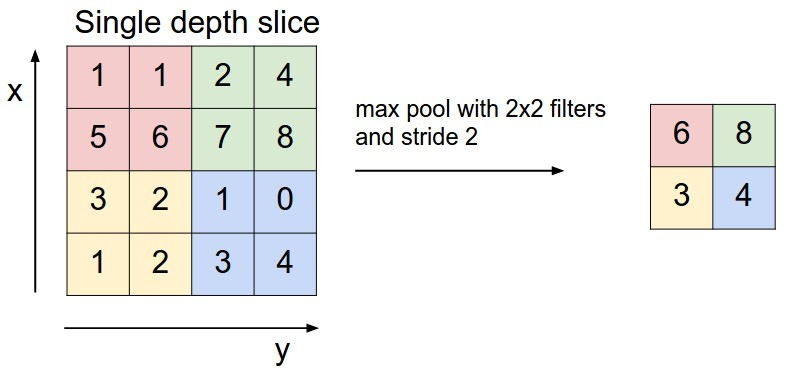
\includegraphics[width=\textwidth]{img/maxpool.jpeg}\caption{Пример max-pooling}
	 	\end{figure}
	 В случае отсутствия max-pooling слоёв применим алгоритм обратного распространения ошибки. Если присутствуют max-pooling слои, то градиенты пробрасываются в ту клетку, на которой достигается максимум, остальные градиенты равны нулю.
	
	В рис.~\ref{pool} ненулевые градиенты будут в точках $(2,2), (2,4), (3,1), (4,4)$.
	
	На практике не встречается использование min-pooling потому что в случае его использования может произойти затухание градиентов.
	
	\section{Свёрточная нейронная сеть}
		В зависимости от постановки задачи после применения свёрточных и pooling слоёв и применения функций активации могут следовать полносвязные или свёрточные  слои. Обычно после применения свёртки следует поэлементное применение функции $\mathrm{ReLU}$, равной $\mathrm{ReLU}(x)=\max(0,x)$ для того, чтобы убрать отрицательные элементы из результатов применения свёрточных слоёв. 
		
		Каждый элемент изображения $M_{ijk}$ показывает интенсивность выбранного пикселя соответствующей координаты и соответствующего канала, в таком случае трудно трактовать отрицательные значения в изображении.
		\newpage
		\begin{figure}[h!]
			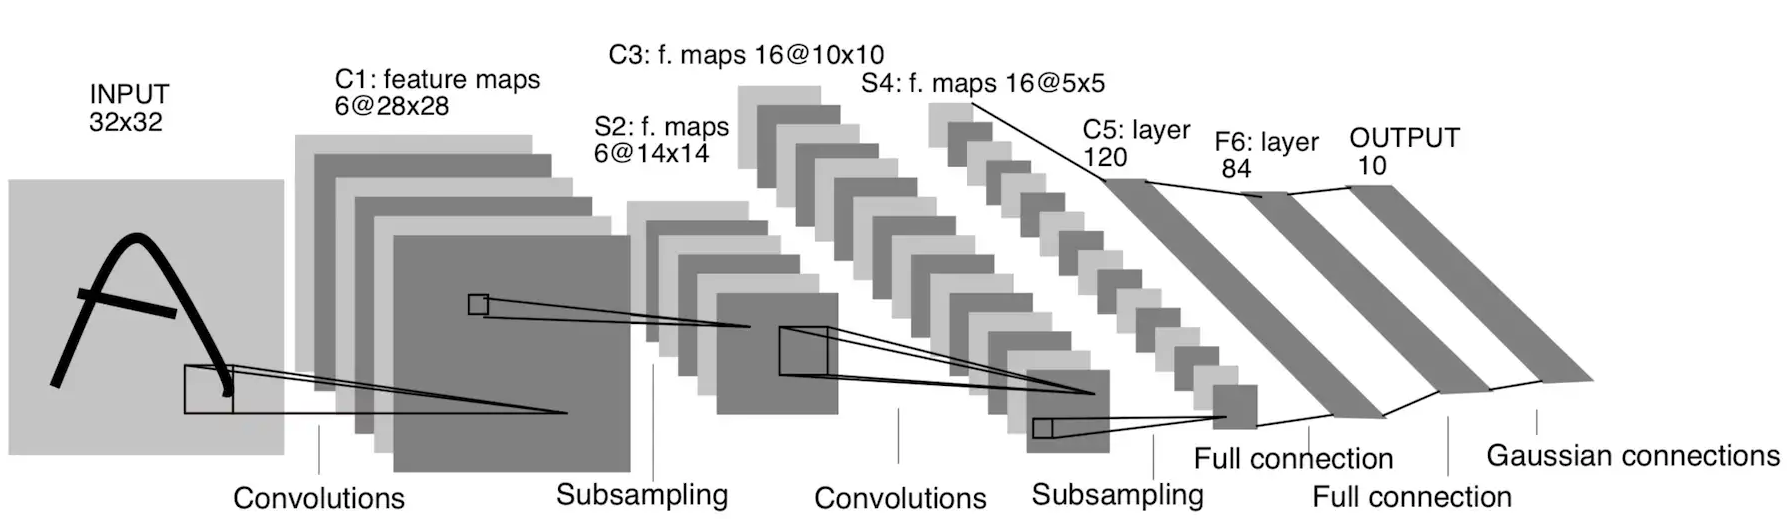
\includegraphics[width=\textwidth]{img/lesnet.png}\caption{Архитектура сети LeNet}
		\end{figure}
		Рассмотрим пример сети LeNet. На первом шаге применяется 6 свёрток размером $5\times5$, затем max-pooling размером $2\times2$, потом 16 свёрток $5\times 5$  и max-pooling $2\times2$, после этого 16 полученных матриц размером $5\times5$ вытягиваются в один вектор, после которого следует два полносвязанных слоя, и на последнем шаге применяется функция активации $\mathrm{softmax}$. В результате получаем вероятность принадлежности одному из десяти классов для каждого класса.
		\section{Улчшения качества свёрточных нейросетей} 
			\subsection{Аугументация}
				Одной из проблем работы с изображениями является малое количество размеченных изображений. Обычно изображения размечаются вручную. Для размножения данных используются аугументации.
				
		\begin{definition}
			Аугументация (Augumentation)~--- увеличение объёма тренировочной выборки с помощью различных афинных преобразований изображений: зеркальное отражение, поворот, сдвиг, изменение масштаба.
		\end{definition}
		
		Также аугументации позволяют улучшить качество предсказания на тестовой выборки. Например, наша задача --- определение дорожных знаков по фотографии. Обучающая выборка состоит из дорожных знаков из справочника (сфотографированы "анфас"). Если обучить модель на выборке без аугументаций, то при рассмотрении реальной фотографии дорожных знаков модель может давать плохие результаты потому что как правило встречаются фотографии с некоторыми дефектами в сравнении с изображениями из обучающей выборки: повороты, размытия, сдвиги. Если рассмотреть аугументированную выборке, то в ней будет больше изображений, похожих на реальные и новая модель сможет предсказывать с большей точностью чем модель, обученная на выборке без аугументаций.
		\newpage 
		\begin{figure}[h!]
			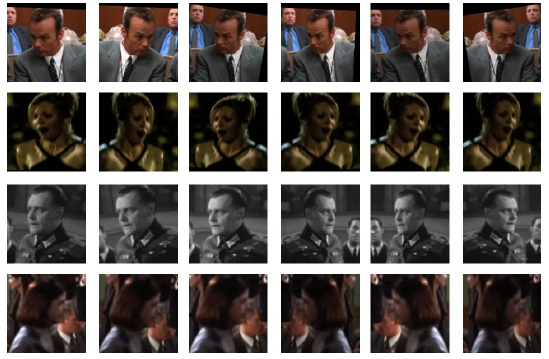
\includegraphics[width=\textwidth]{img/aug.png}\caption{Пример аугументации изображений}
		\end{figure}
	\subsection{ Inception модуль}
		При рассмотрении свёрточного слоя непонятно ядро какого размера следует рассматривать. В качестве решения этой проблемы предлагается внедрение inception модуля в архитектуру сети. Рассмотрим несколько разных комбинаций свёрточных и pooling слоёв, у которых размерности входов и выходов по первым двум координатам (ширине и высоте тензора) равны, пройдём по этим слоям, в результате получим множество тензоров $\{T_i\}_{i=1}^r$, где $w$~--- число рассматриваемых комбинаций свёрток pooling. Каждый тензор $T_i$ имеет размерность $u\times v\times w_i$. На последнем шаге тензоры $T_i$ соединяются вдоль третьей размерности. Рассмотрим некоторый inception модуль на рис.~\ref{inception}. Он состоит из четырёх подмодулей --- различных комбинаций свёрток и/или pooling. Первый подмодуль --- свёртка $1\times1$, второй подмодуль --- свёртка $1\times1$ и $3\times3$, третий состоит из последовательных свёрток $1\times1$ и $5\times5$,  четвёртый из max-pooling $3\times3$ и свёртки $1\times1$. В итоге получаем четыре разных тензора, которые затем соединяем вдоль третьей размерности. 
		\newpage
		\begin{figure}[h!]\label{inception}
			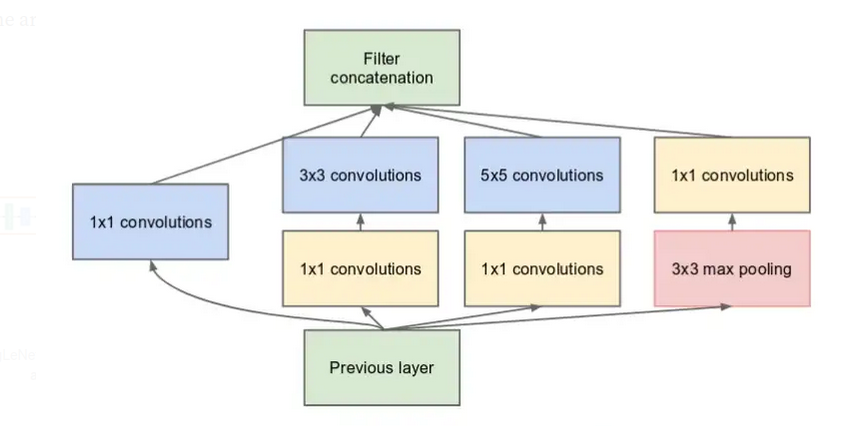
\includegraphics[width=\textwidth]{img/inception.png}\caption{Пример inception модуля}
		\end{figure}
	\section{Выводы}
		Проблемы:
		\begin{itemize}
			\item Необходимость разметки данных для обучения
			\item Большое количество параметром, следовательно долгое обучение, даже на GPU
		\end{itemize}
	Решения:
		\begin{itemize}
			\item Использование размеченных библиотек изображений: ImageNet (14M изображений, 1000 категорий), OpenImages (9М изображений, 60К меток, 20К категория)
			\item Использование модели, обученной на размеченной библиотеке изображений известной архитектуры, например Alexnet, vgg net, Resnet. 
			
		Обычно новые архитектуры публикуются в результате достижения рекордной точности на каком-нибудь соревновании. Например, архитектура vgg 16 показала точность 0.927 на датасете ImageNet на соревновании ImageNet Large Scale Visual Recognition Challenge 2014 и после была опубликована.
		\end{itemize}
		\newpage
		\begin{figure}[h!]
			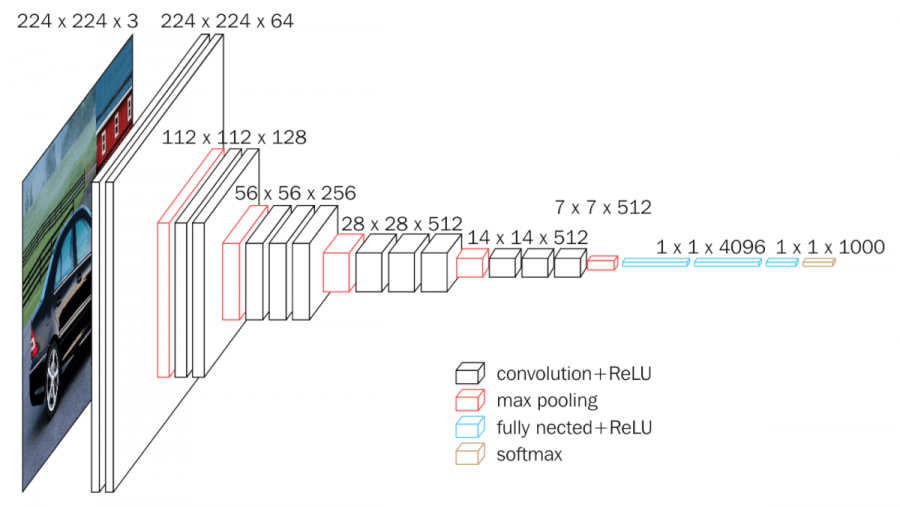
\includegraphics[width=\textwidth]{img/vgg16.png}\caption{Архитектура сети vgg 16}
		\end{figure}
		
		
\section{GAN --- Порождающие состязательные сети}

Порождающие состязательные сети --- алгоритм машинного обучения, входящий в семейство порождающих моделей и построенный на комбинации из двух нейронных сетей: генеративная модель $G$, которая строит приближение распределения данных, и дискриминативная модель $D$, оценивающая вероятность, что образец пришел из тренировочных данных, а не сгенерированных моделью $G$. Обучение для модели $G$ заключается в максимизации вероятности ошибки дискрминатора $D$.

Такие сети используются для следующих целей:

\begin{itemize}
	\item Увеличение разрешения изображений.
	\item Преобразование текста в изображение.
	\item Раскрашивание изображений.
	\item Генерация большего количества данных и заполнение пробелов в них.
\end{itemize}

\begin{figure}[!ht]
	\centering
	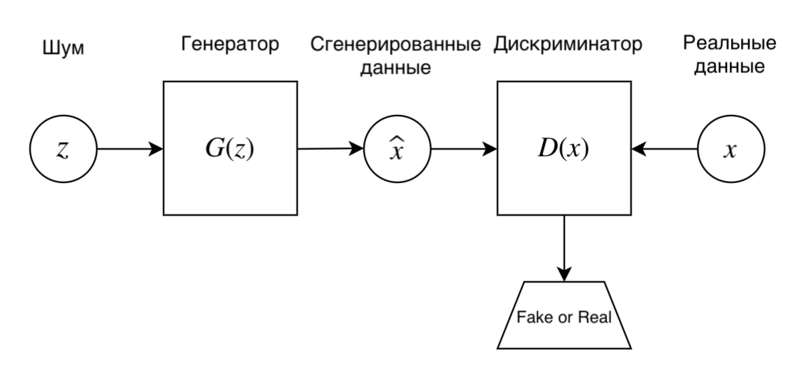
\includegraphics[width=0.7\textwidth]{img/gan_1.png}
	\caption{Схема GAN}
	\label{fig:gan_scheme}
\end{figure}





\subsection{Постановка задачи}

	\begin{figure}[!ht]
	\centering
	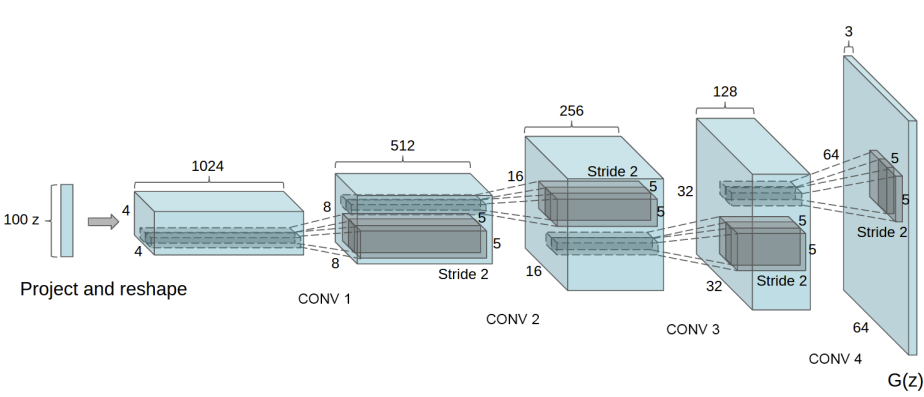
\includegraphics[width=0.7\textwidth]{img/generator.png}
	\caption {Генератор}
	\label{fig:generator}
	\end{figure}

	
	Пусть у нас имеется $d$-мерный набор данных из $n$ индивидов --- $\left\{x_i \in \mathbb{R}^d\right\}_{i=1}^n$; генератор $G$, такой что $G:z \rightarrow x$, $G(z) = x$, где $z\sim p_z(z)$ --- случайный шум из нормального распределения.
	
	Из шума, создаются данные $x$ (например изображение). Цель генератора --- сгенерировать такое изображение $x$, чтобы оно было максимально похоже на изображение из исходных данных $x$.
	
	

	Помимо генератора, в модели GAN существует дискриминатор $D$. По сути, это простой двоичный классификатор с сигмоидальной функцией активации, который в итоге отображает входное изображение в интервал $[0,1]$ следующим образом.
	
		$$D:x\rightarrow [0,1]$$
	
	 Здесь мы предполагаем, что значение дискриминатора 1 будет означать, что $x$ происходит из реального набора изображений, в то время как значение 0 представляет сгенерированное поддельное изображение.
	 
	 $$D(x) = \begin{cases} 1, & \mbox{if } x\mbox{ is real} \\ 0, & \mbox{if } x\mbox{ is generated (fake)} \end{cases}$$
	 
	 
 	$p_{data}(x)$ --- Распределение реальных данных
 	
 	$p_z(z)$ --- Распределение сгенерированных данных
 	
 	\begin{figure}[!ht]
 		\centering
 		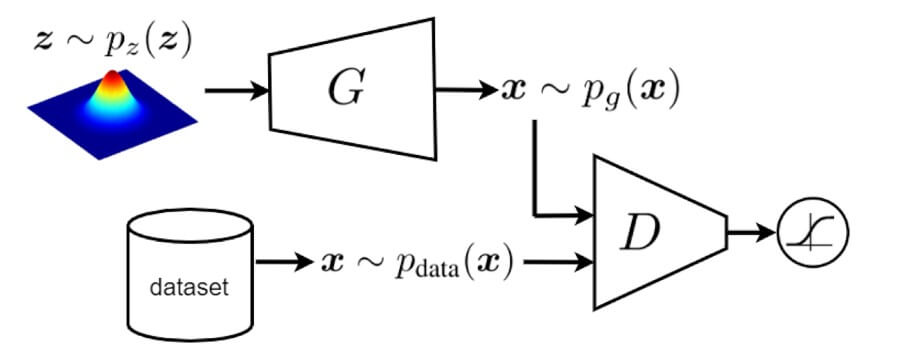
\includegraphics[width=0.8\textwidth]{img/scheme_2.png}
 		\caption {GAN}
 		\label{fig:scheme_2}
 	\end{figure}


Задача:

$$\underset{G}{\min} \underset{D}{\max} V\left(D,G\right) = \underset{x\sim p_{data}}{ \mathbb{E}} \left[\log D(x)\right] + \underset{z\sim p_z}{ \mathbb{E}} \left[\log\left(1-D\left(G(z)\right)\right)\right]$$

Здесь необходимо оптимизировать функцию $V(D,G)$. Она состоит из двух членов. Первый связан с реальными изображениями $x$, которые имеют распределение $p_{data} (x)$. 

Второй связан с изображениями, которые генерируются с помощью источника шума $z$. 

\subsection{Алгоритм обучения}

\begin{enumerate}
	\item Получаем мини-батч ${z_1,...,z_m}$ из распределения $p_z$,
	\item Получаем мини-батч ${x_1,...,x_m}$ из распределения $p_{data}$
	\item Обновляем дискриминатор в сторону возрастания его градиента $$ d_w \leftarrow \nabla_{\gamma_d} \frac{1}{m} \sum\limits_{t=1}^{m}\left[\log D(x_t)\right] +  \left[\log\left(1-D\left(G(z_t)\right)\right)\right]$$
	\item Повторяем шаги 1-3 $k$ раз.
	\item Получаем мини-батч ${z_1,...,z_m}$ из распределения $p_z$
	\item Обновляем генератор в сторону убывания его градиента $$ g_w \leftarrow \nabla_{\gamma_g} \frac{1}{m} \sum\limits_{t=1}^{m} \left[\log\left(1-D\left(G(z_t)\right)\right)\right] $$ 
\end{enumerate}

На практике не всегда удобно использовать уравнение описанной выше. В начале обучения, когда $G$ плохо настроен дискриминатор $D$ может не учитывать объекты, с высокой уверенностью в классификации, так как они сильно отличаются от тренировочного сета, в таком случае $\log\left(1-D\left(G(z)\right)\right)$ стагнирует. Чтобы избежать этого, можно вместо минимизации $\log\left(1-D\left(G(z)\right)\right)$ максимизировать $\log\left(D\left(G(z)\right)\right)$. На рисунке 3 представлена зависимость получаемого изображения от итерации обучения. На рисунке \ref{fig:training} представлена зависимость получаемого изображения от итерации обучения.

\begin{figure}[!ht]
	\centering
	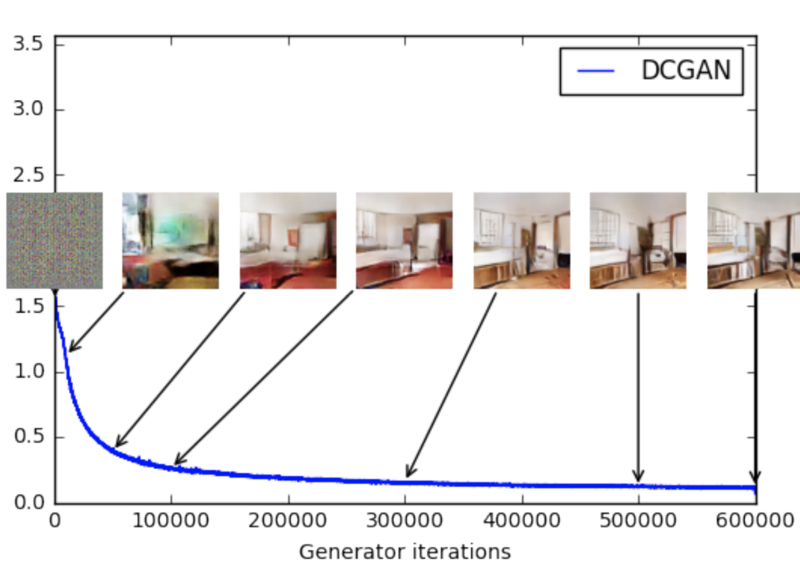
\includegraphics[width=0.7\textwidth]{img/training.png}
	\caption {GAN}
	\label{fig:training}
\end{figure}

\newpage

\subsection{Проблемы обучения GAN}

\begin{itemize}
	\item Генератор  выдает ограниченное количество разных образцов.
	\item Параметры модели дестабилизируются и не сходятся.
	\item Дискриминатор становится слишком сильным, а градиент генератора исчезает и обучение не происходит.
	\item Выявление корреляции в признаках, не связанных (слабо связанных) в реальном мире.
	\item Высокая чувствительность к гиперпараметрам.
\end{itemize}

Cуществуют практические советы, которые могут помочь при обучении GAN'ов. Основными из них являются:

\begin{itemize}
	\item Нормализация данных. Все признаки в диапазоне $[-1,1]$;
	\item Замена функции ошибки для $G$ с $min\log(1-D)$ на $max\log D$, потому что исходный вариант имеет маленький градиент на раннем этапе обучения и большой градиент при сходимости, а предложенный наоборот;
	\item Сэмплирование из многомерного нормального распределения вместо равномерного;
	\item Использовать нормализационные слои (например, batch normalization или layer normalization) в $G$ и $D$;
	\item Использовать метки для данных, если они имеются, то есть обучать дискриминатор еще и классифицировать образцы.
\end{itemize}

\newpage

\section{CGAN --- Условные порождающие состязательные сети}

Условные порождающие состязательные сети --- это модифицированная версия алгоритма GAN, которая может быть сконструирована при помощи передачи дополнительных данных $y$, являющихся условием для генератора и дискриминатора. $y$ может быть любой дополнительной информацией, например, меткой класса, изображением или данными из других моделей, что может позволить контролировать процесс генерации данных. Например, можно подавать параметр $y$, как условие на класс для генерации чисел, похожих на MNIST. Создание таких картинок, в случае передачи картинки в качетсве y является задачей трансляции изображений. Пример работы CGAN на датасете MNIST с метками классов представленных в виде one-hot векторов (рис. \ref{fig:cgan}).



В дискриминаторе $x$ и $y$ представлены как входные параметры. В таком случае задача оптимизации будет выглядеть следующим образом:

$$\underset{G}{\min} \underset{D}{\max} V\left(D,G\right) = \underset{x\sim p_{data}}{ \mathbb{E}} \left[\log D(x|y)\right] + \underset{z\sim p_z}{ \mathbb{E}} \left[\log\left(1-D\left(G(z|y)\right)\right)\right]$$

\begin{figure}[!ht]
	\centering
	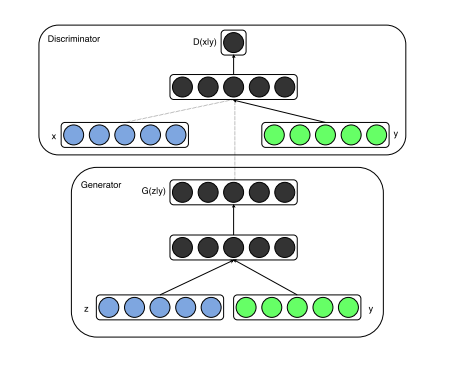
\includegraphics[width=0.8\textwidth]{img/cgan.png}
	\caption {CGAN}
	\label{fig:cgan}
\end{figure}

\newpage

\subsection{DCGAN}

DCGAN --- модификация алгоритма GAN, в основе которых лежат сверточные нейронные сети (CNN). Задача поиска удобного представления признаков на больших объемах не размеченных данных является одной из наибольнее активных сфер исследований, в частности представление изображений и видио. Одним из удобных способов поиска представлений может быть DCGAN. Использование сверточных нейронных сетей напрямую не давало хороших результатов, поэтому было внесены ограничения на слои сверток. Эти ограничения и лежат в основе DCGAN:

\begin{itemize}
	\item Замена всех пулинговых слоев на страйдинговые свертки (strided convolutions) в дискриминаторе и частично-страйдинговые свертки (fractional-strided-convolutions) в генераторе, что позволяет сетям находить подходящие понижения и повышения размерностей;
	\item Использование батчинговой нормализации для генератора и дискриминатора, то есть нормализация входа так, чтобы среднее значения было равно нулю и дисперсия была равна единице. Не стоит использовать батч-нормализация для выходного слоя генератора и входного дискриминатор.
	\item Удаление всех полносвязных скрытых уровней для более глубоких архитектур;
	\item Использование ReLU в качестве функции активации в генераторе для всех слоев, кроме последнего, где используется tanh;
	\item Использование LeakyReLU в качестве функции активации в дискриминаторе для всех слоев.
	
\end{itemize}

\section{StackGAN}

StackGAN --- порождающая состязательная сеть для генерации фото-реалистичных изображений (256x256) исходя из текстового описания. Генерировать фото-реалистичные изображения на обычных GAN сложно, поэтому была придумана двух-этапная модель генерации. Stage-I GAN рисует скетчи с примитивными формами и цветами, основанные на текстовом описании, в низком разрешении. Stage-II GAN принимает на вход изображения с первого этапа и текстовое описание и генерирует изображение в высоком разрешении с фото-реалистичными деталями. Чтобы улучшить разнообразие синтезированных изображений и стабилизировать обучение, вместо CGAN использовался метод Conditioning Augmentation.

Раннее использовались CGAN, поскольку на вход им можно было подавать условия, но просто добавляя слои, увеличивающие размер изображения, достичь хороших результатов не удалось. Поэтому основной задачей было повысить разрешение изображений.

\subsection{Stage I}

Одной из ключевых особенностей StackGAN является Conditioning Augmentation, так как оно позволило расширить количество примеров тренировочного сета, путем небольших случайных изменений в исходных изображениях, что увеличивало многообразие данных. Как показано на картинке, текстовое описание $t$ кодировщиком переводится в векторное представление $\phi_t$ (рис. \ref{fig:stackgan}). Раннее векторное представление нелинейно трансформировалось, чтобы получить скрытые условные переменные, которые подавались на вход генератору, однако простарнство значений скрытых переменных имеет большую размерность, что приводило к разрывам в многообразии данных, что не выгодно для генератора. 

Чтобы избавиться от этого как раз нужно Conditioning Augmentation, которое в отличии от предоставления фиксированных значений переменных выбирает их из нормального распределения $\mathcal{N}\left(\mu(\phi_t), \Sigma(\phi_t)\right)$, где $t$ --- текстовое описание, а $\phi_t$ --- векторное представление . В добавок к уже упомянотому, чтобы сделать многообразие гладким и не переобучиться, нужно добавить регуляризацию,$r = D_{KL} \left(\mathcal{N}\left(\mu(\phi_t), \Sigma(\phi_t)\right)||\mathcal{N}\left(0, I\right)\right)$ (Расстояние Кульбака — Лейблера).

Тренировка дискриминатора $D_0$ и генератора $G_0$:

\vspace{0.1cm}

$ L_{D_0} =  \mathbb{E}_{\left(I_0, t\right)\sim p_{data}} \left[\log D_0 \left(I_0,\phi_t\right)\right] + E_{z\sim t, t\sim p_{data}} \left[\log \left(1- D_0\left(G_0(z,\hat{c_0}), \phi_t\right)\right)\right] $

\vspace{0.2cm}

$ L_{G_0} =  \mathbb{E}_{z\sim t, t\sim p_{data}} \left[\log \left(1- D_0\left(G_0(z,\hat{c_0}), \phi_t\right)\right)\right] + \lambda r $,

где реальное изображение $I_0$ и описание текста $t$ берутся из реального распределения данных $p_{data}$, $z$ --- шумовой вектор.

\begin{figure}[!ht]
	\centering
	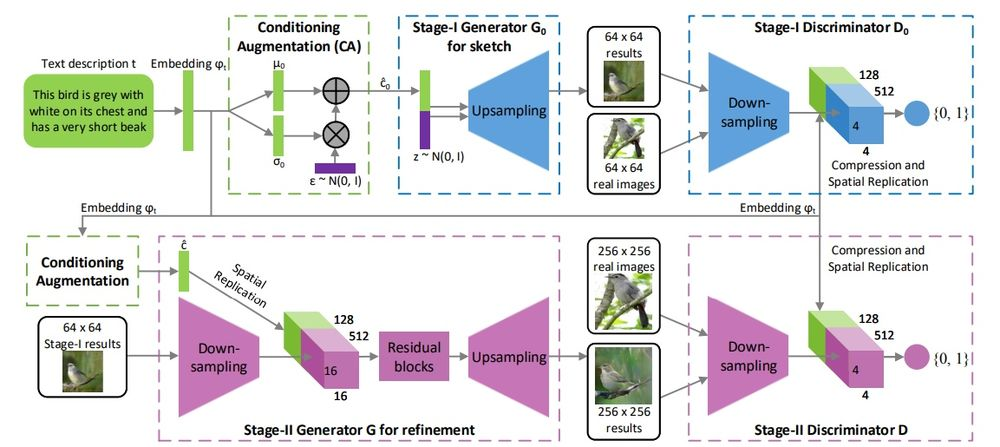
\includegraphics[width=0.8\textwidth]{img/stackgan.jpg}
	\caption {CGAN}
	\label{fig:stackgan}
\end{figure}

\subsection{Stage II}

В изображениях с низким разрешенеим, сгенерированные Stage-I GAN, обычно недостает ярких деталей и могут быть искривления форм, некоторые детали изображения также могут быть опущены на первом этапе. Stage-II GAN построен над Stage-I GAN и принимает на вход его выход, и текстовое описание, чтобы исправить и дополнить изображение. Его дискриминатор и генератор тренируются путем поочередной макисимизации $L_D$ и минимизации $L_G$, как показано в уравнениях:

$$ L_{D} = \mathbb{E}_{\left(I, t\right)\sim p_{data}} [\log D (I,\phi_t)] +  \mathbb{E}_{s_0\sim p_{C_0}, t\sim p_{data}} [\log (1- D(G(s_0,\hat{c}), \phi_t))] $$

$$  L_{G} =   \mathbb{E}_{s_0\sim p_{C_0}, t\sim p_{data}}  \left[\log \left(1- D\left(G(s_0,\hat{c}), \phi_t\right)\right)\right] + \lambda r ,$$

где $s_0 = G_0\left(z, \hat{c_0}\right)$ --- результат работы генератора Stage-I GAN.

\section{LAPGAN}

LAPGAN --- генеративная параметрическая модель, представленная пирамидой лапласианов с каскадом сверточных нейронных сетей внутри, которая генерирует изображения постепенно от исходного изображения с низким разрешением к изображению с высоким. На каждом уровне пирамиды обучается сверточная генеративная модель, используя подход порождающих состязательных сетей. Такая стратегия позволяет декомпозировать задачу генерации изображений на последовательность уровней, что упрощает ее решение.

\begin{itemize}
	\item Пусть $d(\cdot)$ --- операция сжатия изображения размера $j\times j$ так, что новое изображение $d(I)$ имеет размеры $j/2 \times j/2$
	\item $u(\cdot)$ --- операция расширения такая, что $u(I)$ имеет размеры $2j \times 2j$.
\end{itemize}

Тогда пирамида гауссианов имеет вид $\mathcal{G}(I) = \left[I_0,I_1,\ldots, I_k\right]$, где $I_0 = I$, и $I_k$ представляет собой $k$ раз выполненное применение $d(\cdot)$.

Коэффициенты $h_k$ на каждом уровне пирамиды: $$h_k = \mathcal{L}_k(I) = \mathcal{G}_k(I) - u(\mathcal{G}_{k+1}(I)) = I_k - u\left(I_{k+1}\right)$$

\section{Сегментация}
Вновь обратимся к задаче сегментации. 
Пусть $X \in \mathbf{R}^{m \times n \times d} $ --- изображение, $f:X\to Y$, $Y\in[0,1]^{m\times n}$, $Y_{ij}=\Prob(X_{ij}\in\text{segment})$ --- функция, сопоставляющая изображению его маску, segment --- множество принадлежащих сегменту пикселей. Решают задачу \textit{supervised}-методами, то есть требуется наличие размеченных изображений.
Чаще всего для решения этой задачи используется архитектура сети типа \textit{encoder-decoder}.
Как следует из названия, сеть состоит из двух частей --- \textit{encoder}, который последовательно уменьшает размер изображения (кодирует), и \textit{decoder}, который восстанавливает исходное изображение из закодированного (декодирует).
Обычно слои сети симметричны относительно момента перехода от кодировщика к декодировщику и состоят из нескольких наборов сверточных слоёв с батч-нормализацией и функцией активации, но для кодировщика после каждого такого набора также стоит пулинг-слой, а для декодировщика --- наоборот, все это предваряется $\textit{upsampling}$-слоем. На рисунке \ref{ris:image} представлена схема устройства сети SegNet, предназначенной для решения задачи сегментации изображений.

\begin{figure}[h]
\begin{center}
	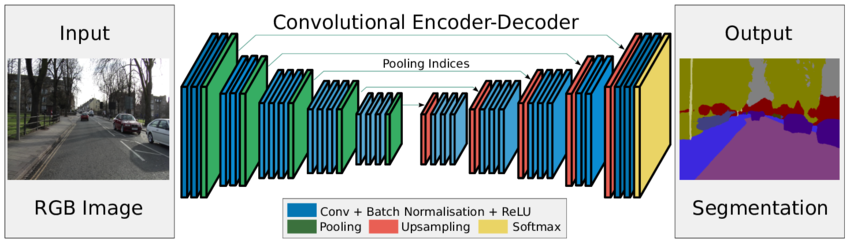
\includegraphics[width=1\textwidth]{img/segnet.png}
\end{center}
\caption{Схема архитектуры сети SegNet}
\label{ris:image}
\end{figure}

\begin{figure}[h]
\begin{center}
	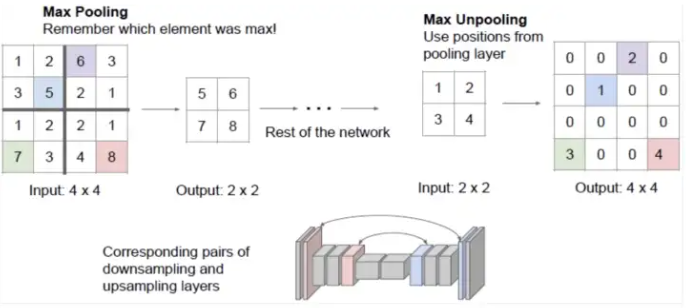
\includegraphics[width=1\textwidth]{img/unpooling.png}
\end{center}
\caption{Иллюстрация работы макс-пулинга и макс-анпулинга.}
\label{ris:image1}
\end{figure}

\begin{figure}[h!]
\begin{center}
	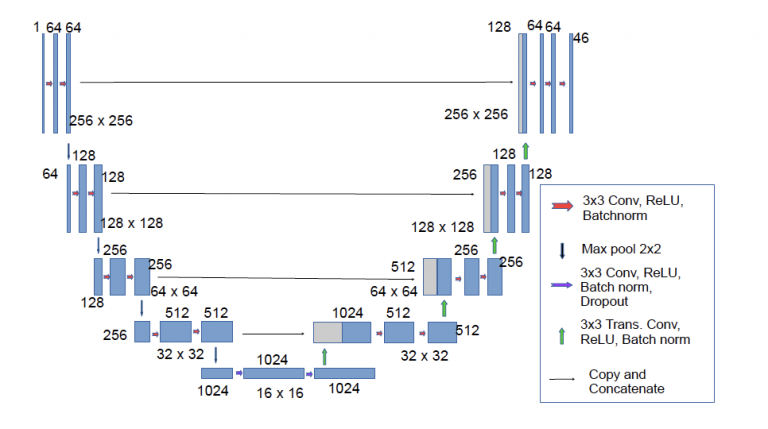
\includegraphics[width=1\textwidth]{img/vanila.png}
\end{center}
\caption{Схема архитектуры сети Vanilla Unet}
\label{ris:image2}
\end{figure}

Обсудим теперь, что же такое $upsampling$-слой. Первый тип $upsampling$ называется $unpooling$.	 Анпулинг пытается выполнить ровно противоположную операцию к пулингу. Можно сделать это разными способами, но чаще всего применяют $max-unpooling$.
Во время выполения макс-пулинга сохраняем позиции, где достигается максимум, и затем используем их в unpooling слое, т.е. помещаем элементы на соотвествующие им позиции, все остальное заполняем нулями (Рис. \ref{ris:image1}).


Одной из возможных модификаций ранее описанной сети является сеть \textit{Vanilla Unet}. 
Особенностью этой сети является использование данных со слоев кодировщика в соответствующих слоях декодировщика (см. Рис. \ref{ris:image2})	. В некоторых случаях эта модификация дает значимое улучшение качества сегментации.

\end{document}
